\chapter{Especificação de Projeto} %% TODO
    Escolhemos descrever o sistema do nosso projeto seguindo o modelo de referência ODP, pois ele apresenta uma forma de simplificar a descrição de sistemas complexos por meio dos seus Pontos de Vista.\cite{odppart1} Sabíamos também que gostaríamos se seguir alguns princípios de projeto, descritos na Tabela \ref{principios_de_projeto}. Esses princípios foram resultado de conversas com engenheiros de software e interessados no projeto, e nos ajudaram a guiar durante a definição dos requisitos de sistema.
    \begin{table}
        \centering
        \caption{Princípios de Projeto}
        \label{principios_de_projeto}
        \resizebox{\textwidth}{!}{%
        \begin{tabular}{|l|p{10cm}|}
            \hline
            Princípio de Projeto                 & Descrição \\ \hline
            Ambientes de curta duração           & O desenvolvedor deve ser capaz de criar e deletar ambientes com rapidez e facilidade                                 \\ \hline
            Visualização de fluxos complexos     & O desenvolvedor deve ser capaz de visualizar o resultado de suas requisições HTTP e mensagens Kafka                  \\ \hline
            Ambiente parecido com o local        & O desenvolvedor deve ter uma experiência de desenvolvimento similar com o ambiente de sua máquina                    \\ \hline
            Esconde complexidade de configuração & O desenvolvedor não deve precisar conhecer a configuração dos serviços que ele precisa disponíveis no ambiente dele. \\ \hline
        \end{tabular}
        }
        \legend{Fonte: os autores}
    \end{table}
	\section{Ponto de Vista da Empresa}
	    As empresas que podem se beneficiar do nosso projeto devem ter alguma semelhança com o processo de negócio de desenvolvimento e entrega de novas funcionalidades, descritos respectivamente nas Figuras \ref{fig:build-ci} e \ref{fig:automated-deploy}. O primeiro processo descreve como uma alteração de código por um desenvolvedor gera novas imagens Docker, que são guardadas em um catálogo chamado \textit{Docker Registry}. Exemplos de \textit{Docker Registry} são o DockerHub e o Quay.io. Já o segundo processo, descreve como uma imagem desses catálogo é implantada de forma automatizada pelo Servidor de Entrega Contínua.
	    \begin{figure}[htb]
    	    \centering
    	    \caption{Processo de Entrega Contínua - Construção da imagem Docker}
    	    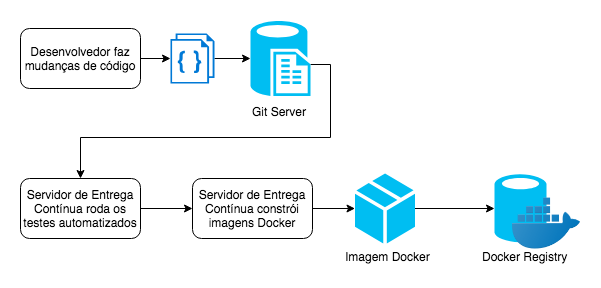
\includegraphics[scale=0.7]{pictures/especificacao-de-projeto/build-ci.png}
    	    \legend{Fonte: os autores}
    	    \label{fig:build-ci}
	    \end{figure}
	    \begin{figure}[htb]
    	    \centering
    	    \caption{Processo de Entrega Contínua - Implantação automatizada}
    	    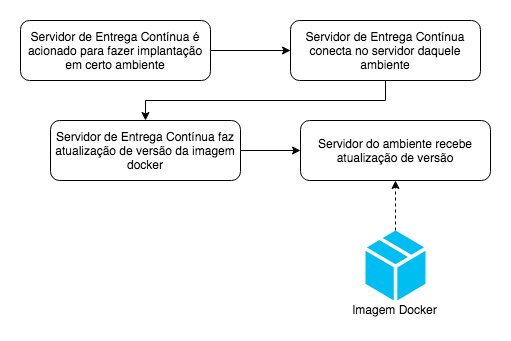
\includegraphics[scale=0.7]{pictures/especificacao-de-projeto/automated-deploy.png}
    	    \legend{Fonte: os autores}
    	    \label{fig:automated-deploy}
	    \end{figure}
	\section{Ponto de Vista da Informação}
	    O objetivo dessa seção é apresentar a organização das informações por todos os componentes do sistema. A Figura \ref{fig:info-contexts} representa os três principais contextos onde as informações são modeladas, e como é o fluxo de informações. 
	    \begin{figure}[htb]
    	    \centering
    	    \caption{Contextos de informação e seu fluxo}
    	    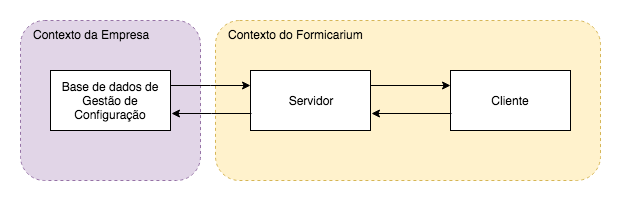
\includegraphics[scale=0.67]{pictures/especificacao-de-projeto/information-contexts.png}
    	    \legend{Fonte: os autores}
    	    \label{fig:info-contexts}
	    \end{figure}
	    \subsection{Contexto da Empresa}
	        O contexto da empresa refere-se a uma base de dados pré-existente capaz de fornecer as configurações de uma aplicação dado o ambiente: teste, homologação e produção, tradicionalmente. Assim, a modelagem dessa base de dados pode ser arbitrária em relação ao sistema do Formicarium.
	    \subsection{Contexto do Formicarium}
	        \subsubsection{Servidor}
	        A Figura \ref{fig:info-server} representa a modelagem da configuração necessária para rodarmos uma aplicação. Note que uma aplicação pode possuir múltiplas interfaces e pode constituir por múltiplos contêineres. Isso permite maior flexibilidade na implantação e modelagem de aplicações.
	        \begin{figure}[htb]
        	    \centering
        	    \caption{Modelagem das Informações no Servidor}
        	    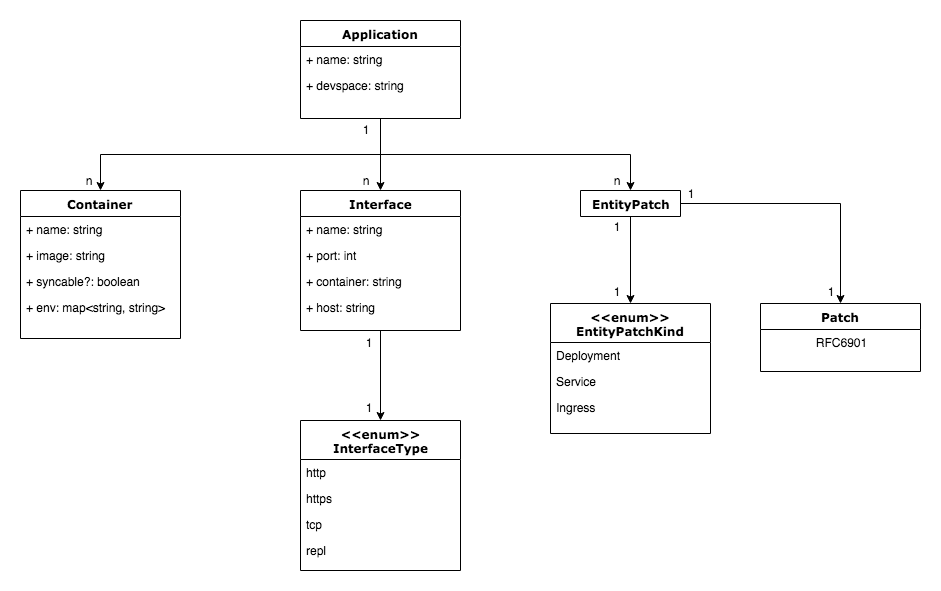
\includegraphics[scale=0.40]{pictures/especificacao-de-projeto/info-server.png}
        	    \legend{Fonte: os autores}
        	    \label{fig:info-server}
	        \end{figure}
	        \subsubsection{Cliente}
	            
	\section{Ponto de Vista da Computação}
	    O Ponto de Vista da computação está diretamente ligado a distribuição. Não diz respeito aos mecanismos de interação, mas decompõe o sistema em objetos capazes de realizar funções e interagir por interfaces bem definidas \cite{odppart1}.
	    \subsection{Arquitetura de Referência} %% TODO: Leal
	        A arquitetura deste projeto compartilha conceitos e mecanismos com arquiteturas de Plataformas como Serviço (\textit{Platform as a Service}), em particular a arquitetura da Heroku.
	        
	        A Heroku se descreve da seguinte forma: "Heroku é uma plataforma de nuvem baseada em um sistema de contêineres gerenciado, com integração a serviços de dados e um poderoso ecossistema, para implantação e execução de aplicações modernas. O \textit{Heroku Developer Experience} é uma abordagem centrada na aplicação para entrega de software, integrada com as mais populares ferramentas e fluxos de trabalhos atuais." (\citeauthor{herokuplatform}, \citeyear{herokuplatform}).
	        
	        A arquitetura da Heroku têm diversos componentes, destacados a seguir aqueles relevantes ao projeto.
	        \subsubsection{Plataforma}
	            A plataforma consiste no sistema operacional, \textit{runtime} da linguagem e bibliotecas associadas. Esses subcomponentes já mudaram com o tempo. Hoje, a plataforma da Heroku adota o Ubuntu como sistema operacional, o que permite suporte a múltiplas linguagens de programação como Java, Clojure, Python, Ruby e Node.js.\cite{herokucloud}
	            
	            Para o desenvolvedor usuário da plataforma, é necessário prover um arquivo Procfile que representa um processo UNIX, e provê o ambiente de execução da aplicação, quantidade de réplicas e modularidade. Além disso, a plataforma fornece uma interface de linha de comando com métodos análogos ao UNIX, como representado na Figure \ref{fig:herokucli}. Através dessa interface, também é possível gerenciar atualizações da aplicação.\cite{herokucloud}
        	    \begin{figure}[htb]
            	    \centering
            	    \caption{Interface de Linha de Comando da Heroku}
            	    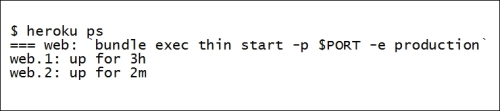
\includegraphics[scale=0.75]{pictures/especificacao-de-projeto/heroku-ps.jpg}
            	    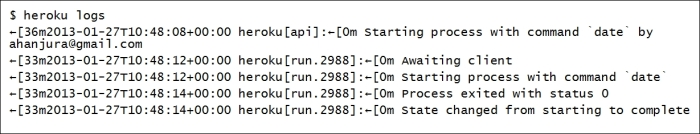
\includegraphics[scale=0.75]{pictures/especificacao-de-projeto/heroku-logs.jpg}
            	    \legend{Fonte: Heroku Cloud Application Development}
            	    \label{fig:herokucli}
        	    \end{figure}
        	    
	        \subsubsection{Mecanismo de Roteamento de Requisições}
	            Além de gerenciar os processos da aplicação, a plataforma também fornece um domínio sobre 
	            \texttt{herokuapp.com}. Quando uma requisição HTTP chega à infraestrutura da Heroku, a malha de roteamento direciona para o servidor onde o contêiner, que a Heroku chama de \textit{dyno}, está em execução.\cite{herokucloud}
        	    \begin{figure}[htb]
            	    \centering
            	    \caption{Representação da Malha de Roteamento}
            	    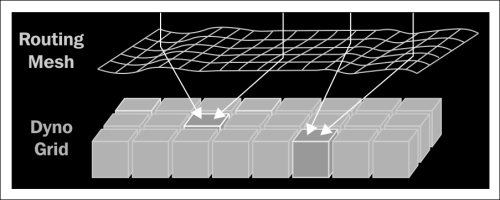
\includegraphics[scale=2.5]{pictures/especificacao-de-projeto/heroku-routing.jpg}
            	    \legend{Fonte: Heroku Cloud Application Development}
            	    \label{fig:herokurouting}
        	    \end{figure}
	        \subsubsection{Infraestrutura de \textit{Add-ons}}
	            \textit{Add-ons} são uma maneira de terceiros fornecerem extensões das funcionalidades da plataforma. Exemplos possíveis são bancos de dados, serviços de mensageria, email e SMS. A Figura \ref{fig:herokuaddons} mostra a necessidade de uma interface entre a plataforma e o provedor de serviços terceiros. \cite{herokucloud}
	            \begin{figure}[htb]
            	    \centering
            	    \caption{Infraestrutura de \textit{Add-ons} da Heroku}
            	    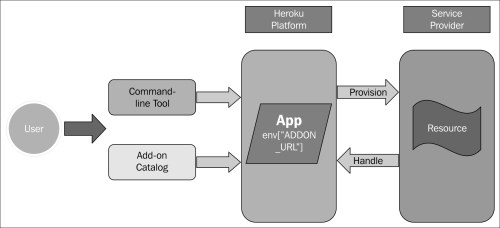
\includegraphics[scale=2.5]{pictures/especificacao-de-projeto/heroku-addons.jpg}
            	    \legend{Fonte: Heroku Cloud Application Development}
            	    \label{fig:herokuaddons}
        	    \end{figure}
        \subsection{Diferenças e Arquitetura do Projeto}
            O principal ponto de diferença, é claro, são os objetivos das plataformas. Enquanto a Heroku se propõe a ser uma plataforma que roda aplicações em ambiente de produção, o Formicarium é focado em ambientes de desenvolvimento dentro das empresas.
            
            \subsubsection{Plataforma}
                O Formicarium usa o Kubernetes como plataforma, e assim, abstrai os requisitos de sistema operacional. No entanto, é altamente recomendado utilizar Nodes com sistema operacional Linux. Trabalhando com contêineres Docker também permite maior flexibilidade no suporte a linguagens de programação, uma vez que, caso não exista ainda um contêiner com o ambiente apropriado para ele, é possível construir esse contêiner sem grandes dificuldades.
                
                O Kubernetes também fornece um modelo de informação inicial para trabalharmos: os objetos da API Kubernetes como \textit{pods}, \textit{deployments} e \textit{ingresses}. No entanto, esses objetos foram modelados no contexto de operação e implantação de software, e não ambientes de desenvolvimento. Isso faz com que seja mais trabalhoso do que necessário. Assim, desenvolvemos uma modelagem mais apropriada, já descrita no Ponto de Vista da Informação.
                
            \subsubsection{Mecanismo de Roteamento de Requisições}
                Para o roteamento de requisições, o Formicarium têm requisitos bem menos exigentes que a Heroku, uma vez que o todo o fluxo é dado pelos desenvolvedores. Assim, é possível substituir a malha de roteamento, que exige uma infraestrutura de rede mais complexa, por um \textit{reverse proxy}.
                
                O funcionamento do \textit{reverse proxy} se dá pelo direcionamento da requisição com base no \textit{hostname}. Isso permite que um domínio DNS represente diversas aplicações.
                
                \begin{figure}[htb]
            	    \centering
            	    \caption{Roteamento de Requisições no Formicarium}
            	    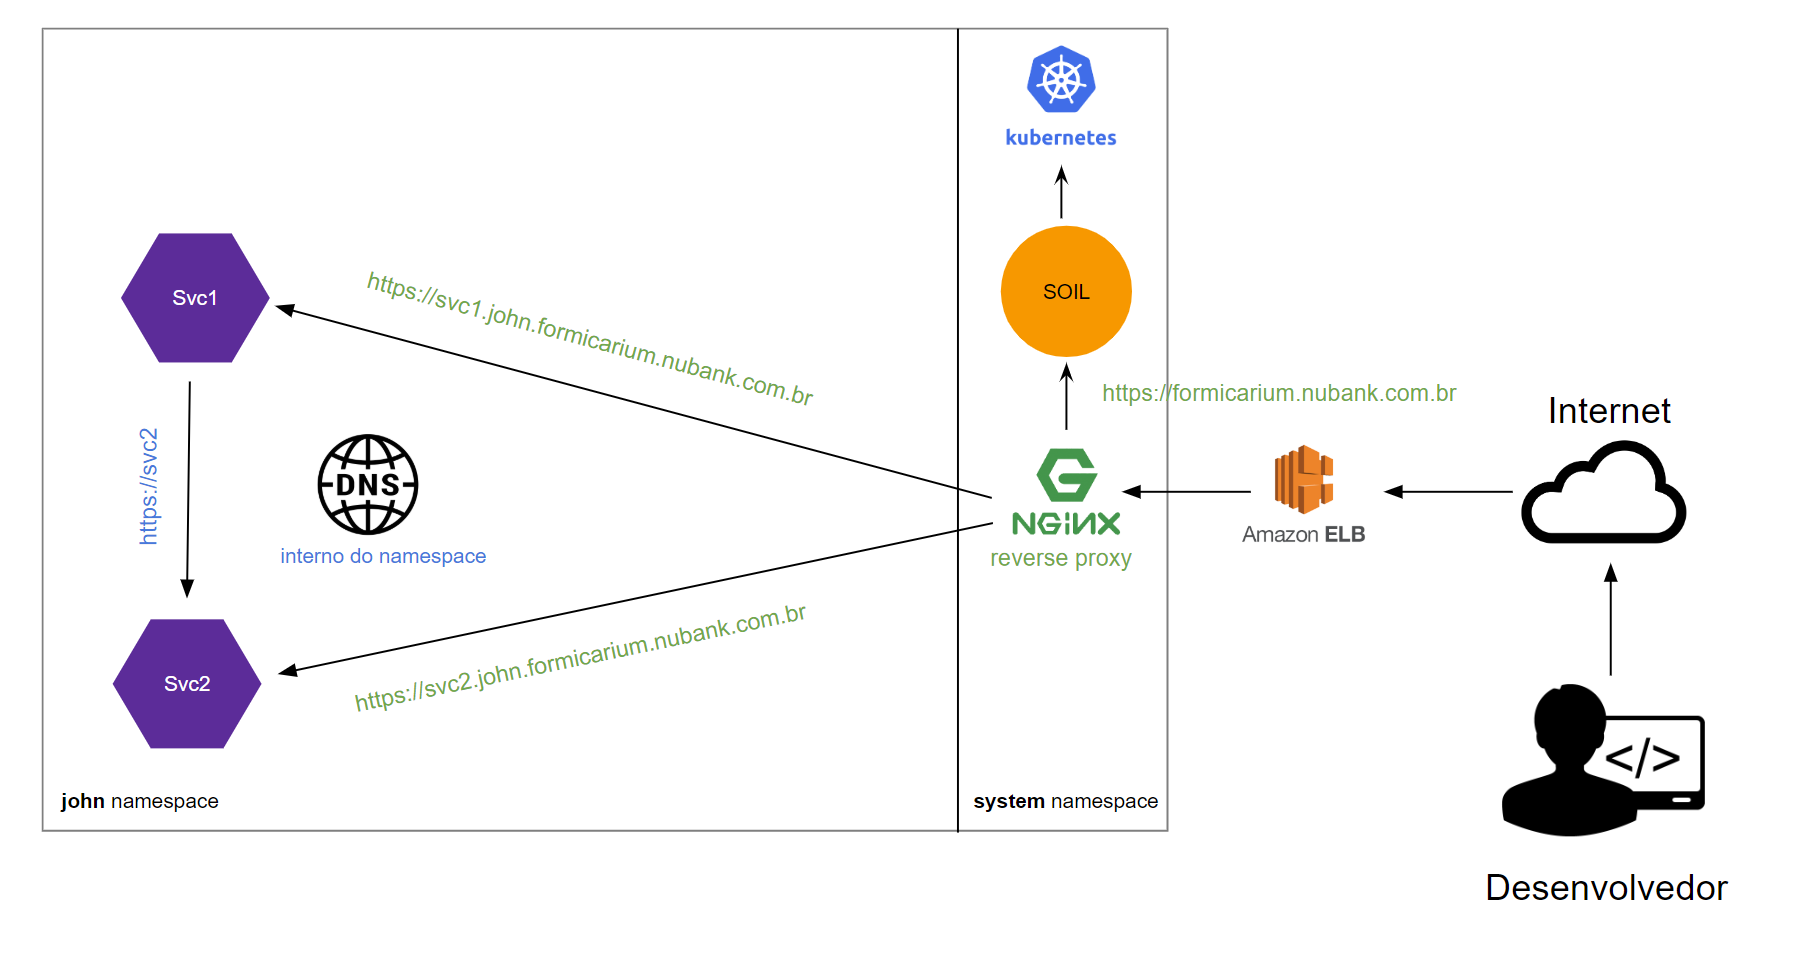
\includegraphics[scale=0.32]{pictures/especificacao-de-projeto/fmc-routing.png}
            	    \legend{Fonte: os autores}
            	    \label{fig:fmcrouting}
        	    \end{figure}
        	    
    	    \subsubsection{Desacoplamento Empresa e Formicarium}
    	        O Formicarium não possui uma infraestrutura de \textit{add-ons}. No entanto, é necessário uma forma de desacoplamento entre os modelos de configuração das aplicações pela empresa e da configuração necessária para criação dessas aplicações na plataforma.
    	        
    	        Assim, a empresa é responsável por desenvolver um serviço de configuração das aplicações. Configura-se então o Formicarium para acessar esse serviço, de forma que, para o desenvolvedor, a configuração é transparente.
    	        
    	        \begin{figure}[htb]
            	    \centering
            	    \caption{Desacoplamento Empresa e Formicarium}
            	    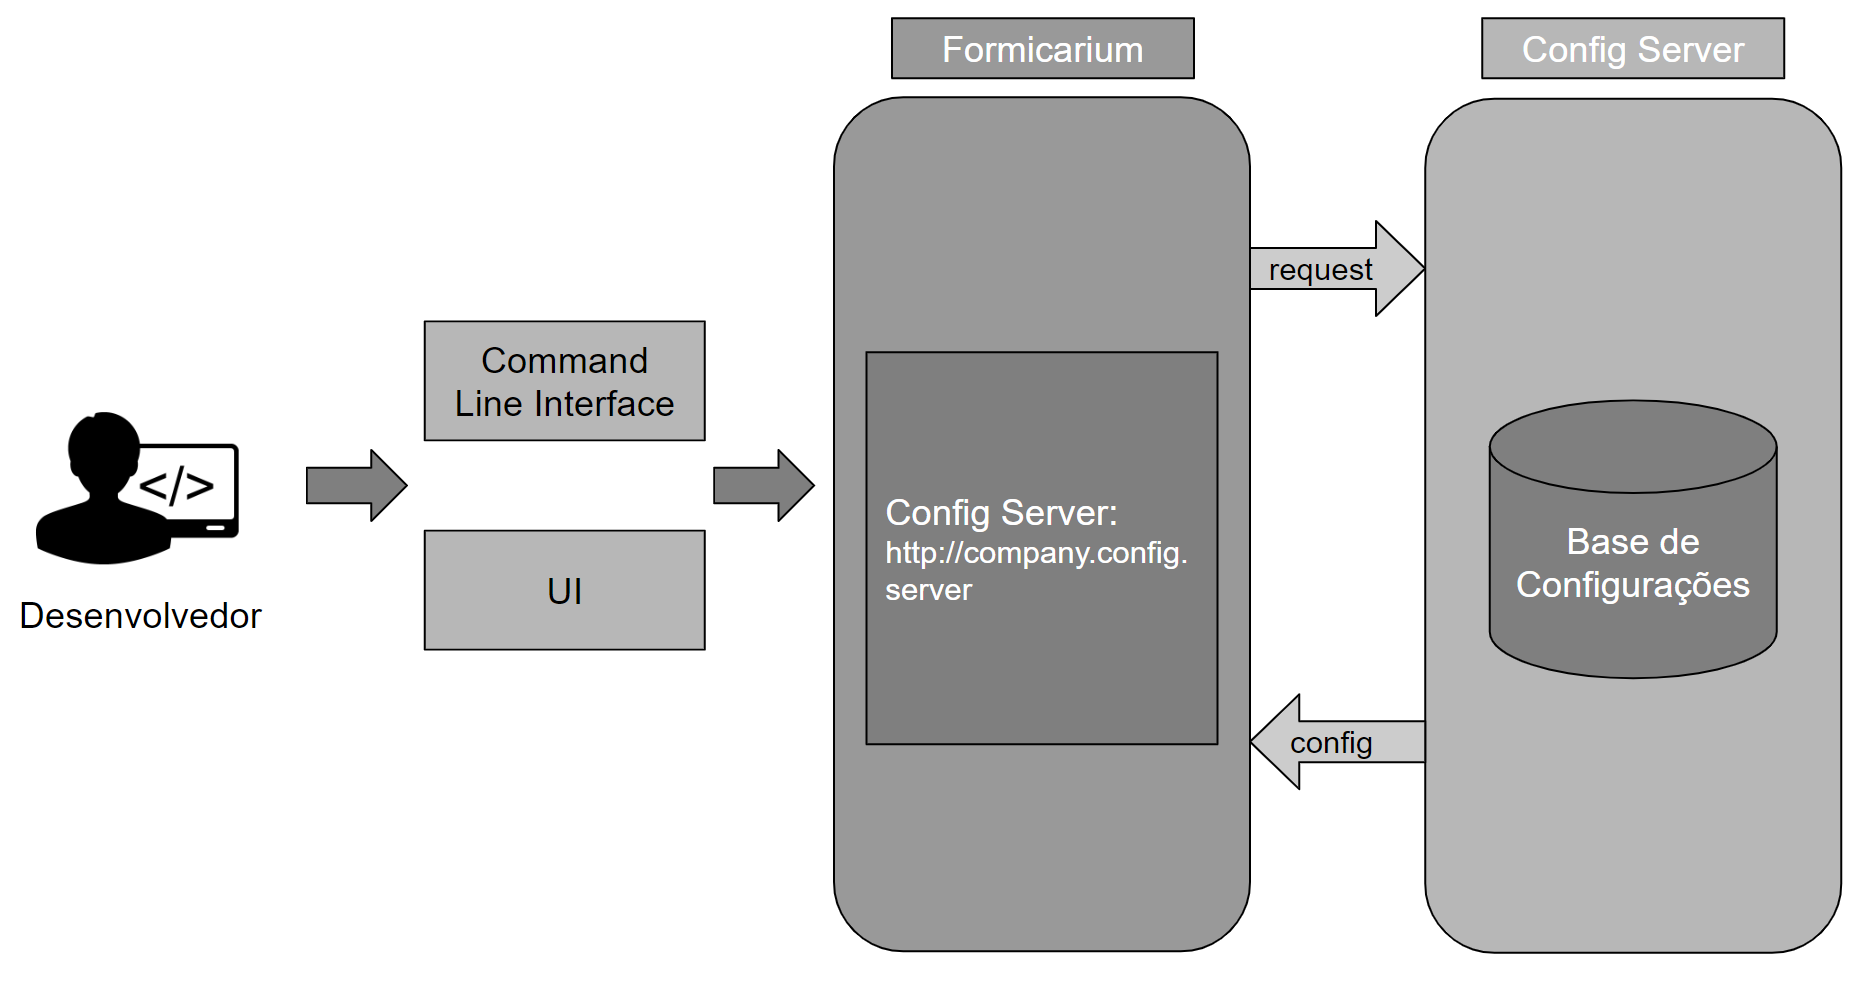
\includegraphics[scale=0.24]{pictures/especificacao-de-projeto/fmc-decoupling.png}
            	    \legend{Fonte: os autores}
            	    \label{fig:fmcdecoupling}
        	    \end{figure}
        	    
        	\subsubsection{Infraestrutura de Depuração}
        	    Para a depuração de problemas nas aplicações, o Formicarium possui comandos assim como a plataforma da Heroku. No entanto, dado que esse é o foco da plataforma, é necessário mais do que simplesmente inspeção de logs.
        	    
        	    Para isso, há um componente especializado em agregar informações relevantes de depuração. Esse componente é criado junto com os Devspaces, e possuem um armazenamento efêmero.
        	    
    	        
	\section{Ponto de Vista da Engenharia}
	    
	\section{Ponto de Vista da Tecnologia}